\documentclass[12pt,a4paper,twoside]{article}

\usepackage[utf8]{inputenc}
%\usepackage[latin1]{inputenc} 
\usepackage[T1]{fontenc}
\usepackage{lmodern} % load a font with all the characters
\usepackage{gensymb}
\usepackage{mathtools,xparse}

\usepackage{amsthm}

\usepackage{amsmath}

\usepackage{amssymb}
\usepackage{pdfpages}
\usepackage{mathrsfs}

\usepackage{graphicx}

\usepackage{hyperref}

% inclure the numéro du chapitre dans les équations
\numberwithin{equation}{subsection}

\DeclarePairedDelimiter{\abs}{\lvert}{\rvert}
\DeclarePairedDelimiter{\norm}{\lVert}{\rVert}
\begin{document}
% indentation des paragraphes
\setlength{\parindent}{0cm}

\newpage
\tableofcontents

\newpage
\section{Introduction}

cet oeuvrage est un résumé. 

faire le lien entre différentes sciences.

Des résultats développés dans une partie sont utilisés dans d'autres parties.

\newpage
\section{Algèbre}

\subsection{Logarithme}
\subsubsection{Relations}
Fonction et fonction inverse (réciproque)
\begin{eqnarray}
e^n=x\\
ln(x)=n\\
ln(x^a)=a\cdot n
\end{eqnarray}

\subsubsection{Changement de base}
\begin{eqnarray}
log_{n}(x)=\frac{ln(x)}{ln(n)}=a\\
n^a=x
\end{eqnarray}

\subsection{Produits remarquables}
Théorème de Binôme : 
\begin{equation}
(a+b)^n=\sum_{k=0}^{n}a^{n-k}b^k
\end{equation}
\subsection{Equation de degré 2}
\begin{equation}
a x^2+ bx +c =0
\end{equation}

Discriminant

\begin{equation}
\Delta = b^2-4\cdot a \cdot c
\end{equation}

3 possibilités : 

\begin{enumerate}
	\item $\Delta > 0 $ :  Il y a deux solutions réelles.\\ $x_{1,2}=\frac{-b \pm \sqrt{\Delta}}{2 a}$
	\item $\Delta = 0 $ : Une solution réelle.
	$x=\frac{-b}{2 a}$
	\item $\Delta < 0 $ : Il y deux solutions complexes.\\
	$x_{1,2}=\frac{-b\pm i \sqrt{\abs{\Delta}}}{2 a}$
\end{enumerate}
\subsection{Equation degré 3 : Méthode de Cardan}

Inverse d'une matrice :

Produit de convolution

\subsection{Suites \& Séries}

suite de finonesci//
suite arithmétique

\begin{equation}
\sum_{k=1}^{n}k=\frac{n(1+n)}{2}
\end{equation}
\begin{equation}
\lim \frac{1-r^n}{1-r}
\end{equation}

\subsection{Nombres complexes}

\subsubsection{Utilité}
résoudre des équations qui donne des réusltats impossible dans le domaine réel. exemple $\sqrt{-1}$.\\
\subsubsection{Définition}
Partie réelle, partie imaginaire,\\

Multiplication par le conjugué\\

\subsubsection{Résolution d'équations imaginaires}

\subsection{Série et transformée de Fourier}
Continue :
\begin{equation}
F(\nu)=\int_{-\infty}^{\infty} f(t) e^{-2 i \pi \nu t} dt
\end{equation}

Discrète : 

\subsection{Transformée de Laplace}

\newpage
\section{Equations différentielles}
degré 1,2, solution homogène, solution particulière,
coefficients constants/variables. 
equ diff partielle : résolution avec fourier/Laplace

\newpage
\section{Algèbre linéaire}
\begin{equation}
A^{-1}=()
\end{equation}

décomposition LU, \\
Equation caractéristique, vecteur propre, valeur propre

\newpage
\section{Analyse numérique}

Dérivée numérique, intégrale numérique, equation différentielle partielle numérique (espace, temps), résolution , précision, \\

progressive, rétrograde

\newpage
\section{Cinématique multi-corps}
Euler, Newton\\
quadrilatère article\\
Boucle vectorielle fermée\\
Méthode de Newton-Raphson\\
equilibrage des arbres\\
\newpage

\newpage
\section{Cryptologie}
cours Collège\\
Codage numérique :\\
\url{https://fr.wikipedia.org/wiki/Fonction_OU_exclusif}\\

\newpage
\section{Systèmes de coordonnées}
coordonnées cartésiennes, polaires, cylindriques, sphériques, ....\\
\subsection{Coordonnées cylindriques}
\begin{eqnarray}
r=\rho \cdot \vec{e}_{\rho}+z \cdot \vec{e}_z\\
v=\dot{\rho} \cdot \vec{e}_{\rho} + \rho \cdot \dot{\Phi}\cdot \vec{e}_{\Phi}+\dot{z}\cdot \vec{e}_z\\
a=(\ddot{\rho}-\rho \cdot \Phi^2)\vec{e}_{\rho}+(\rho \cdot \ddot{\Phi}+2 \cdot \dot{\rho}\cdot \dot{\Phi})\vec{e}_{\Phi}+\dot{z}\cdot \vec{e}_z
\end{eqnarray}

\subsection{Coordonnées sphériques}

\begin{eqnarray}
r=r \cdot \vec{e}_r\\
v=r \cdot \vec{e}_{r} + r \cdot \dot{\theta}\cdot \vec{e}_{\theta}+r \cdot \Phi\cdot sin(\theta) \cdot \vec{e}_{\Phi}\\
a=(\ddot{r}-r \cdot \dot{\theta}^2-r\cdot \dot{\Phi}^2 \cdot sin^2(\theta))\vec{e}_{r}+\\
(r \cdot \ddot{\theta}+2 \cdot \dot{r}\cdot \dot{\theta}-r\cdot \dot{\theta}^2 \cdot sin(\theta)cos(\theta))\vec{e}_{\theta}+\\
(r \cdot \ddot{\Phi} \cdot sin(\theta)+2 \cdot \dot{r} \cdot \dot{\Phi} \cdot sin(\theta)+2 \cdot r \cdot \dot{\Phi} \cdot \dot{\theta} \cdot cos(\theta))\cdot \vec{e}_{\Phi}
\end{eqnarray}

\newpage
\section{Géométrie}

Pour vérifier qu'un triangle ABC est rectangle en un point C, on vérfie que le produit scalaire de AC et BC soit nulle


\subsection{Triangle quleconque}
Propriétés : \\



\begin{equation}
\alpha+\beta+\gamma=\pi
\end{equation}

Théorème d'Al-Kashi



Triangle avec cotés a,b,c et angles $\alpha$ $\beta$ $\gamma$. $\alpha$ opposé à a, $\beta$ à b, $\gamma$ à c. 
\begin{equation}
\frac{b}{a}=\frac{\beta}{\alpha}....
\end{equation}
Théorème du sinus
\begin{equation}
\frac{a}{sin(\alpha)}=\frac{b}{sin(\beta)}=\frac{c}{sin(\gamma)}=2\cdot r
\end{equation}
$r$ : rayon du cercle circonscrit. 
Théorème du cosinus
\begin{equation}
a^2=b^2+c^2 - 2 b c cos(\alpha)
\end{equation}
Aire du triangle
\begin{equation}
S=\frac{1}{2}\cdot a b sin(\gamma)=2r^2sin(\alpha)sin(\beta)sin(\gamma)
\end{equation}
\subsection{Trigonométrie}
relations
\begin{eqnarray}
cos^2(x)+sin^2(x)=1\\
\frac{cos(x)}{sin(x)}
\end{eqnarray}
\begin{equation}
tan(x)=\frac{cos(x)}{sin(x)}
\end{equation}

\begin{equation}
cotan(x)=\frac{1}{tan(x)}
\end{equation}

\subsection{Norme}
Norme euclidienne, et les autres types de normes

\subsection{Vecteurs}
Une grandeur qui a une direction, un sens et une intensité
\begin{equation}
\vec{AB}=\vec{OB}-\vec{OA}=
\begin{bmatrix}
x_B-x_A \\
y_B-y_A\\
z_B-z_A
\end{bmatrix}
\end{equation}
Norme vecteur
\begin{equation}
\norm{\vec{B}}=\sqrt{x_B^2+y_B^2+z_B^2}
\end{equation}
Vecteur dimension n :
\begin{equation}
\norm{\vec{B}}=\sqrt{x_B^2+y_B^2+z_B^2}
\end{equation}
\begin{equation}
\norm{\vec{u}}=\sqrt{\sum_{1}^{n}u_i^2}
\end{equation}
normalisation d'un vecteur : on modifier un vecteur de façon à ce que sa norme valle 1 :

\begin{equation}
\vec{B}_{normalisé}=\frac{\vec{B}}{\norm{\vec{B}}}= \frac{1}{\sqrt{x_B^2+y_B^2+z_B^2}} \begin{bmatrix}
x_B\\
y_B\\
z_B
\end{bmatrix}
\end{equation}

Multiplication par un scalaire : 
\begin{equation}
k\cdot \vec{B}= \begin{bmatrix}
k\cdot x_B\\
k\cdot y_B\\
k\cdot z_B
\end{bmatrix}
\end{equation}
Distributivité 
\begin{equation}
k\cdot (\vec{A}+\vec{B})=k\cdot \vec{A}+k\cdot\vec{B}=
\end{equation}

Le vecteur $\vec{v}$ est colinéaire à $\vec{u}$ s'il existe un scalaire $k$ tel que :  
\begin{equation}
\vec{v}=k\cdot \vec{u}
\end{equation}

Combinaison linéaire
\begin{equation}
\vec{u}=\sum_{1}^{n} n_i \cdot \vec{x_i}
\end{equation}
3 vecteurs coplanaires : un des vecteurs est la combinaison linéaire des deux autres
\subsection{Base}
des vecteurs forment une base s'ils sont linéairement indépendants. (non colinéaire)

\subsection{Produit scalaire}
Projection d'un vecteur sur un autre.

\begin{eqnarray}
\vec{A} \cdot \vec{B}=\norm{\vec{A}} \cdot \norm{\vec{B}} \cdot cos(\theta)\\
\vec{A} \cdot \vec{B}= 
\begin{bmatrix}
x_A \\
y_A\\
z_A
\end{bmatrix}
\begin{bmatrix}
x_B \\
y_B\\
z_B
\end{bmatrix}
=x_A x_B + y_A y_B + z_A z_B
\end{eqnarray}

Si deux vercteurs sont perpendiculaires, $theta$ vaut 90$\degree$ :
\begin{equation}
\vec{A} \cdot \vec{B}=0
\end{equation}

\subsection{Volume}

\subsection{Produit vectoriel}

\subsubsection{Définition}
Le produit vectoriel de deux vecteurs $\vec{A}$ et $\vec{B}$ résulte en un vecteur qui leur est perpendiculaire. La norme de ce vecteur est égale à l'aire du parallélogramme formé par les vecteurs $\vec{A}$ et $\vec{B}$. (schéma)
\subsubsection{Relation}
\begin{eqnarray}
\vec{A} \otimes \vec{B}=\norm{A} \norm{B} sin(\theta)\\
\vec{A} \otimes \vec{B}=
\begin{bmatrix}
x_A \\
y_A\\
z_A
\end{bmatrix}
\otimes
\begin{bmatrix}
x_B \\
y_B\\
z_B
\end{bmatrix}= 
\begin{bmatrix}
y_A z_B - z_A y_B \\
-x_A z_B + z_A x_B\\
x_A y_B - y_A x_B
\end{bmatrix}
\end{eqnarray}

Pour connaître la direction du vecteur résultant, on utilise la règle des trois doigts. 

Si les deux vecteurs sont parallèles, l'angle , 
\begin{equation}
\vec{A} \otimes \vec{B}=0
\end{equation}


\subsubsection{Propriétés}
pas commutatif,
\begin{eqnarray}
\vec{A} \otimes \vec{B}=-(\vec{B} \otimes \vec{A})\\
\end{eqnarray}
 distributif par rapport à l'addition, \\
 
 pas associatif

\subsection{Equations dans l'espace}
\subsubsection{Dans le plan}
Equation paramétrique d'une droite\\
\begin{equation}
ax+by+c=0\\
\end{equation}
Equation paramétrique d'une droite\\
\begin{equation}
y=a\cdot x+b\\
\end{equation}


Forme usuelle : 
\begin{equation}
ax+by+c=0\\
\end{equation}


Equation algébrique d'une droite :
\begin{equation}
D=\{(x,y) \in \mathbb{R} ^2 |ax+by+c=0\}
\end{equation}

\subsubsection{Dans l'espace}
\paragraph{Droite}
Equation algébrique d'une droite :

\begin{equation}
D={(x,y,z) \in \mathbb{R} ^3 |ax+by+cz+d=0}
\end{equation}

Equation vectorielle d'une droite :

\begin{eqnarray}
\left\{
\begin{array}{l c c r}   
x &=& a t+ x_P &\\
y &=& b t+ x_P & \\
z &=& c t + z_P & 
\end{array}\right.
t \in \mathbb{R}
\end{eqnarray}
Avec 
$P=
\begin{bmatrix}
x_p \\
y_P\\
z_P
\end{bmatrix}
$ 
un point de la droite et $\vec{u}=\begin{bmatrix}
a\\ b\\ c
\end{bmatrix}$ vecteur directeur de la droite.\\

Une autre forme de l'équation vectorielle :

\begin{equation}
(D_1):
\begin{bmatrix}
x \\
y\\
z
\end{bmatrix}
=
\begin{bmatrix}
x_p\\
y_p\\
z_p\\
\end{bmatrix}
+
\lambda
\begin{bmatrix}
a\\
b \\
c
\end{bmatrix}
; \lambda \in \mathbb{R}
\end{equation}
\paragraph{Plan}
Equation paramétrique d'un plan :
\begin{equation}
ax+bx+cz+d=0
\end{equation}
Avec $\vec{u}=\begin{bmatrix}
a\\ b\\ c
\end{bmatrix}$ verteur normale au plan.\\
Equation vectorielle :
\begin{equation}
(\Pi):
\begin{bmatrix}
x \\
y\\
z
\end{bmatrix}
=
\begin{bmatrix}
x_p\\
y_p\\
z_p\\
\end{bmatrix}
+\lambda
\begin{bmatrix}
m_1\\
m_2 \\
m_3
\end{bmatrix}
+ \gamma
\begin{bmatrix}
n_1\\
n_2 \\
n_3
\end{bmatrix}; (\lambda,\gamma) \in \mathbb{R}
\end{equation}
$\vec{m}$ et $\vec{n}$ appartiennent au plan $\Pi$.
\paragraph{Cercle}

\begin{equation}
r^2=x^2+y^2
\end{equation}
Paramétrisation :
\begin{equation}
C =
\begin{bmatrix}
r \cdot cos(\theta) \\
r \cdot sin(\theta)\\
z
\end{bmatrix}
\end{equation}
Equation cercle, sphère, couronne, solénoide, courbes, splines, ....\\

résumer le tout dans un tableau. 

\subsection{Allignements}
pour vérifier si des points sont alignés, il y a deux méthodes :\\
Méthode 1 : 
\begin{enumerate}
	\item Calculer les vecteurs directeurs entre chaques deux points
	\item Normaliser ces vecteurs
	\item Comparer
	\item Les vecteurs normalisés doivent être égaux
\end{enumerate}

Méthode 2 : 
\begin{enumerate}
	\item Choisir deux points
	\item Créer une droite avec une équation vectorielle
	\item Vérifier que les autres points appartiennent à la droite
\end{enumerate}

\subsection{Intersections}
Intersection entre deux éléments : égaliser les expressions.
\medbreak
Exemple : soit deux droites $D_1$ et $D_2$ :
\begin{equation}
(D_1):
\begin{bmatrix}
x \\
y\\
z
\end{bmatrix}
=
\begin{bmatrix}
x_p\\
y_p\\
z_p\\
\end{bmatrix}
+
\lambda
\begin{bmatrix}
a\\
b \\
c
\end{bmatrix}
; \lambda \in \mathbb{R}
\end{equation}
\begin{equation}
(D_2):
\begin{bmatrix}
x \\
y\\
z
\end{bmatrix}
=
\begin{bmatrix}
u_p\\
v_p\\
w_p\\
\end{bmatrix}
+
\gamma
\begin{bmatrix}
d\\
e \\
f
\end{bmatrix}
; \gamma \in \mathbb{R}
\end{equation}
On trouve l'intersection en posant :

\begin{equation}
(D_1)\cap(D_2):
\begin{bmatrix}
x_p\\
y_p\\
z_p\\
\end{bmatrix}
+
\lambda
\begin{bmatrix}
a\\
b \\
c
\end{bmatrix}
=
\begin{bmatrix}
u_p\\
v_p\\
w_p\\
\end{bmatrix}
+
\gamma
\begin{bmatrix}
d\\
e \\
f
\end{bmatrix}
\end{equation}
en recherchant les solutions pour $\gamma$ et $\lambda$
\medbreak
Intersection entre deux plans donne une droite : 
\begin{eqnarray}
\left\{
\begin{array}{l c r}
	a_1x+b_1 y+c_1 z+d_1 &=&0\\
	a_2 x+ b_2 y + c_2 z + d_2 &=&0
\end{array}
\right.
\end{eqnarray}

Intersection entre droite et plan donne un point :


\subsection{Projections}
calculer la distance entre deux éléments\\
Distance entre un point et une droite, droite et un plan, point à un plan, ....
\subsection{Calculs volume}

calculer volume surface, d'une fonction.

Volume (rotation de la fonction autour d'une droite, ...., avec une intégrale) : considérer la fonction comme un rayon et calculer le volume d'un cercle d'épaisseur $dx$.\\
\paragraph{Autour de l'axe X}
\begin{equation}
V=\int_{a}^{b}\pi \cdot f(x)^2 \cdot dx
\end{equation}
\paragraph{Autour de l'axe Y}
(à confirmer)
\begin{eqnarray}
V=\int_{a}^{b}\pi \cdot x^2 \cdot dy\\
dy=\frac{df(x)}{dx}\cdot dx
\end{eqnarray}
\paragraph{Autour d'un axe quelconque}
.....
\subsection{Calculs surface}
\paragraph{Surface}
surface : délimité par deux fonctions $g(x)$ et $f(x)$. 
\begin{equation}
S=\int_{a}^{b} (f(x)-g(x)) \cdot dx
\end{equation}
\newpage
\section{Mathématiques}
moyenne : moyenne aritmétique, et autre type de moyenne ....

\newpage
\section{Matériaux}
loi de Hooke :
\begin{equation}
\sigma = \epsilon \cdot E 
\end{equation}
Contrainte à la rupture 

\begin{equation}
\sigma=\frac{K_{1c}}{\sqrt{\pi e}}
\end{equation}


\newpage
\section{Mécanique}


\subsection{Cinématique}
\subsubsection{MRU}
Mouvement rectiligne uniforme :
\begin{eqnarray}
a(t)=0\\
v(t)=v=const\\
x(t)=v \cdot t + x_0
\end{eqnarray}

\subsubsection{MRUA}
Mouvement rectiligne uniformément accéléré :
\begin{eqnarray}
a(t)=a=const\\
v(t)=a \cdot t+v_0\\
x(t)=\frac{1}{2} \cdot a \cdot t^2+v_0 \cdot t + x_0
\end{eqnarray}

\subsubsection{MCU}
\subsubsection{MCUA}


\subsection{Equations d'équilibre}
1er loi de Newton \\


2ème loi de Newton, 
\begin{equation}
\Sigma F= m*a
\end{equation}

3ème loi de Newton : \\

action = réaction \\

Equation couple
\begin{equation}
\Sigma M=I*\alpha
\end{equation}

\subsection{Mécanique Lagrangienne}
q : variables d'état d'un système
\begin{equation}
L(q,\dot{q})=\sum E_{cin}(q,\dot{q}) - \sum E_{pot}(q,\dot{q})
\end{equation}
$E_{cin}$ : Energie cinétique de translation et de rotation.\\
$E_{pot}$ : Energie potentielle

Equation de Lagrange :
\begin{equation}
\frac{d}{dt}(\frac{\delta L}{\delta \dot{q}_i})-\frac{\delta L}{\delta q_i}=0
\end{equation}


\subsection{Centre de masse et moment d'inertie}
Centre de masse d'un corps solide:

\begin{equation}
x_G=\frac{\int x \cdot dm}{\int dm}
\end{equation}

Pour un assemblage de plusieurs corps solides :
\begin{equation}
x_G=\frac{\sum x_i \cdot m_i}{\sum m_i}
\end{equation}

Centroïde d'une courbe
\begin{equation}
x_G=\frac{\int x \cdot dA}{A}
\end{equation}

Centroïde d'une surface 
\begin{equation}
x_G=\frac{\int x \cdot dl}{l}
\end{equation}

Centroïde d'un volume
\begin{equation}
x_G=\frac{\int x \cdot dV}{V}
\end{equation}

Moment d'inertie d'un corps solide : 
\begin{equation}
I=\iiint d^2 dm=\iiint d^2 \rho dV
\end{equation}
Assemblage 
\begin{equation}
I=\sum r_i^2 \cdot m_i
\end{equation}

Théorème de Huygens-Steiner : 
\begin{equation}
I=I_G+m\cdot m^2
\end{equation}

Quelques formules d'inertie : \\
\begin{center}
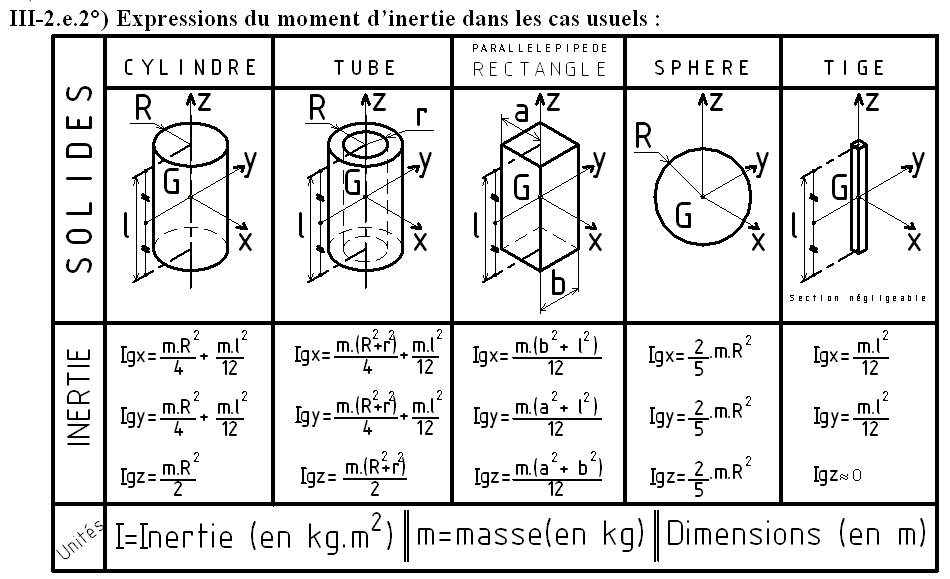
\includegraphics[scale=0.65]{MomentDinerties.png}
\end{center}
\url{http://www.bonne-mesure.com/moment_d_inertie.php}\\

Rayon de giration
\begin{eqnarray}
I_G=m \cdot k_g^2 \Rightarrow k_G=\sqrt{\frac{I_G}{m}}\\
k^2=k_G^2+d^2
\end{eqnarray}

Thm du sinus + (schéma du triangle)
\begin{equation}
\frac{a}{sin(\alpha)}=\frac{b}{sin(\beta)}=\frac{c}{sin(\gamma)}
\end{equation}
Thm cosinus
\begin{equation}
c^2=a^2+b^2-2 \cdot a \cdot b \cdot cos(\gamma)
\end{equation}

\subsection{Quantité mouvement, moment cinétique}
théorème quantité de mouvement : TAero, début Part 2\\
\begin{equation}
\iint_\Sigma [(\vec{p} \vec{n})+\rho \vec{V}(\vec{V} \vec{n})]d\sigma
\end{equation}
cette intégrale donne la force de poussée. \\
moment cinétique, théorème implusion\\
\url{https://fr.wikipedia.org/wiki/Quantit%C3%A9_de_mouvement}

\newpage
\section{Mécanique des fluides}

Equation de Bernoulli : \\



Pour calculer le $C_x$ ou le $C_z$, il faut calculer la circulation $\Gamma$ autour du profil. Ces deux coefficients dépendent de l'angle d'incidence $\alpha$.

\begin{eqnarray}
\Gamma = \oint v ds\\
C_{L}=\frac{2 \Gamma}{t v_{\infty}}
\end{eqnarray}
$s$ est le contour du profil.\\


Aile d'avion :
\begin{eqnarray}
C_z=2 k_{AR} \alpha\\
C_x= C_{x_p} + \frac{(C_z)^2}{\pi AR}\\
AR=\frac{b^2}{S}\\
k_{AR}=(\frac{\pi}{1+\frac{2}{AR}})^{\frac{1}{2}}
\end{eqnarray}
S : surface des ailes. b : envergure. AR : allongement relatif. $C_{x_p}$ : \footnote{Cours Techniques aéronautiques, Jean-Michel Schulz}\\

Finesse :
\begin{equation}
f=\frac{C_z}{C_x}
\end{equation}
On trouve la finesse max en cherchant $\frac{\delta f}{\delta \alpha}$
Force de portance (Lift) :
\begin{equation}
F_z= \frac{1}{2}*\rho S V^2 C_z
\end{equation}

Force de traînée (Drag) : 
\begin{equation}
F_x= \frac{1}{2}*\rho S V^2 C_x
\end{equation}

Nombre de Reynolds, viscosité statique, viscosité dynamique
\begin{equation}
Re=\frac{V l}{\mu}
\end{equation}

\newpage
\section{Mécaniques des fluides/aérodynamique}
Force de frottement visqueux
\begin{equation}
\vec{F}=-k\cdot \vec{v}=-k\cdot 
\begin{bmatrix}
\dot{x} \\
\dot{y}\\
\dot{z}
\end{bmatrix}
\end{equation}

Force de frottement laminaire
\begin{eqnarray}
\vec{F}=-k \cdot \eta \cdot \vec{v_{rel}}\\
\vec{v_{rel}}=\vec{v_{objet}}-\vec{v_{fluide}}
\end{eqnarray}

Force de frottement turbulant
\begin{eqnarray}
\vec{F}= \frac{1}{2} \rho_{fluide} \cdot S \cdot C_x \cdot \abs{v_{rel}}^2\\
\vec{v_{rel}}=\vec{v_{objet}}-\vec{v_{fluide}}
\end{eqnarray}
$S$ : aire de la prise à l'air \\
$C_x$ : coefficient de traînée\\


Force de portance (lift) :
\begin{equation}
F_z=\frac{1}{2}*\rho_{gaz}*S*C_z*V^2
\end{equation}
$\rho_{gaz}$ : masse volumique du gaz $[\frac{kg}{m^3}]$\\
$S$ : Section de référence $[m^2]$\\
$C_z$ : coefficient de portance $[-]$\\
$V$ : vitesse de l'objet $[\frac{m}{s}]$\\

Force de trainée (drag) :
\begin{equation}
F_x=\frac{1}{2}*\rho_{gaz}*S*C_x*V^2
\end{equation}
$\rho_{gaz}$ : masse volumique du gaz $[\frac{kg}{m^3}]$\\
$S$ : Section de référence $[m^2]$\\
$C_x$ : coefficient de trainée $[-]$\\
$V$ : vitesse de l'objet $[\frac{m}{s}]$\\


\newpage
\section{Mécanique des structures}

Loi de Hooke linéaire
\begin{equation}
F=k\cdot \Delta x
\end{equation}

\subsection{Traction/compression}
\begin{equation}
\sigma=\frac{F}{S}
\end{equation}

\begin{equation}
\epsilon=\frac{\delta L}{l}
\end{equation}

\begin{equation}
\epsilon=\frac{\sigma}{E}
\end{equation}

\subsection{Effort tranchant}
\subsection{Flexion}

\subsection{Torsion}

Méthode flexion 3 points\\
Poutre encastrée


\newpage
\section{Mécanique vibratoire}
modèle simple, pendule simple, amortissement, equation différentielle, solutions réelles, solutions complexes, ....
exercice suspension vhc : système roue amortisseur/ressort -> fonction de transfert

\subsection{Système à un degré de liberté}

Ocillateur simple : une masse avec un ressort et un amortissement

Equation du mouvement :
\begin{equation}
m \ddot{x} + c \dot{x}+k x =0
\end{equation}
qu'on peut écrire différemment. 
\begin{equation}
\ddot{x} + 2\zeta \omega_0 \dot{x}+\omega_0^2  x =0
\end{equation}

\begin{eqnarray}
\omega_0=\sqrt{\frac{k}{m}}\\
\zeta=\frac{c}{c_r}\\
c_r=2 m \omega_0=2\sqrt{km}
\end{eqnarray}
$c_r$ : constante d'amortissement critique. 

Solution : $x(t)=C \exp^{\lambda t}$

\newpage
\section{Physique}
Force gravitationnelle
\begin{equation}
\vec{F}_g=G\cdot \frac{m_1 \cdot m_2}{d^2} [N]
\end{equation}
Gravité terrestre : 
\begin{equation}
g=G\cdot \frac{m_{terre}}{(Rayon_{terre}+altitude)^2}[\frac{m}{s^2}]
\end{equation}

Frottement sec
\begin{equation}
F=\mu \cdot F_n [N]
\end{equation}
$\mu$ : coefficient de frottement $[-]$\\
La force normale $F_n$ est perpendiculaire à $F$.(schéma)\\


Pression d'Archimède :
\begin{equation}
P=\rho \cdot g \cdot h [Pa]
\end{equation}

Dilatation unidirectionnelle :
\begin{equation}
\Delta L=L_0 \cdot \alpha  \cdot \Delta T
\end{equation}
$\alpha$ : coefficient de dilation thermique $[-]$\\
$\Delta T$ : Différence de température $[K]$\\

Dilatation volumique : 
\begin{equation}
\Delta V=V_0 \cdot \beta \cdot \Delta T
\end{equation}
$\beta \approx 3\cdot \alpha$

\subsection{Lois de conservation}
\subsubsection{Quatité de mouvement}
\begin{equation}
\vec{P}=m \cdot \vec{v}
\end{equation}
\begin{equation}
\sum P_{i}=\sum m_i \cdot v_i= \sum P_i '=\sum m_i ' \cdot v_i '
\end{equation}
\subsubsection{Energie}
\begin{equation}
\sum E_{initiale}=\sum E_{finale}
\end{equation}

\begin{eqnarray}
E_{cin}^{translation}=\frac{1}{2} \cdot m \cdot v^2\\
E_{cin}^{rotation}=\frac{1}{2} \cdot I_G \cdot \omega^2\\
E_{pot}^{gravité}=m \cdot g \cdot h\\
E_{pot}^{élastique}=\frac{1}{2} \cdot k \cdot x^2
\end{eqnarray}

\subsubsection{Moment cinétique}
Corps solide
\begin{equation}
\vec{L}=I \cdot \vec{\omega}
\end{equation}
Pt matériel
\begin{equation}
\vec{L}=\sum \vec{GP_i}*m\cdot \vec{r}_i
\end{equation}
Théorème de Huygens-Steiner
\begin{equation}
I=I_G+M \cdot d^2
\end{equation}

\begin{equation}
\vec{L}_c=\vec{L}_G+ \vec{CG} * m \cdot \vec{v}=\vec{L}_G'+ \vec{CG} * m \cdot \vec{v}'=\vec{L}_c'
\end{equation}

\subsection{Lois de distribution}
vitesse
\begin{equation}
\vec{v}_p=\vec{v}_G+\vec{\omega}*\vec{GP}
\end{equation}
accélération
\begin{equation}
\vec{a}_p=\vec{a}_G+\vec{\dot{\omega}}*\vec{GP}+\vec{\omega}*(\vec{\omega}*\vec{GP})
\end{equation}

\subsection{Chocs}
Chocs élastique : conservation des 3 lois. 
\begin{eqnarray}
\frac{dE_{cin}}{dt} =0
\end{eqnarray}
Chocs inélastique/mou :
\begin{eqnarray}
\frac{dE_{cin}}{dt} \neq 0\\
\frac{d P^{tot}}{dr}=\vec{F}_{ext}\\
\frac{d L^{tot}}{dr}=\vec{M}_{0}^{ext}
\end{eqnarray}

\newpage
\section{Statistique}
\subsection{Combinatoire}
Combinaison : 
\begin{equation}
C(x,y)=\begin{bmatrix}
x\\
y
\end{bmatrix}=\frac{x!}{(x-y)!\cdot y!}
\end{equation}


Permutation
\begin{equation}
P(x)=x!
\end{equation}
Répartition d'un groupe de x dans des groupes de y et z éléments.

\begin{eqnarray}
x=y+z\\
P^x_{y,z}=\frac{x!}{y! \cdot z!}
\end{eqnarray}
\subsection{***********}

moyenne
\begin{equation}
\mu=\sum x_i \cdot P_i
\end{equation}

\begin{equation}
\mu = \frac{1}{n}\sum x_i
\end{equation}

variance
\begin{equation}
v=\sum (x_i-\mu)^2\cdot P_i
\end{equation}
\begin{equation}
v=\frac{1}{n} \sum (x_i-\mu)^2
\end{equation}
écart-type
\begin{equation}
\sigma=\sqrt{v}=\sqrt{\sum (x_i-\mu)^2\cdot P_i}
\end{equation}

Espérance (cas discret)
\begin{equation}
E(X)=\mu=\sum_{i=1}^{n}x_i\cdot P_i
\end{equation}
Jeu équitable si $E(X)=0$. avec bénifice $E(X)>0$

\newpage
\section{Régulation}

Laplace, Fonction de transfert, Boucle de régulation : ouverte, fermée

\newpage
\section{Thermodynamique}
\subsection{Définitions}
Loi des gaz parfaits
\begin{eqnarray}
PV=nRT\\
Pv=rT
\end{eqnarray}
$P$ : Pression du gaz $[Pa]$\\
$V$ : Volume du gaz $[m^2]$\\
$v$ : Volume spécifique $[\frac{m^2}{kg}]$\\
$n$ : nombre de mole $[mol]$\\
$R$ : Constante des gaz 8.314 $[\frac{J}{K \cdot K}]$\\
$r$ : Constante massique d'un gaz \\
$T$ : Température $[K]$\\


Equation de Van der Waals :
\begin{equation}
p \cdot (V-)=n R T
\end{equation}

Energie interne d'un gaz :
\begin{equation}
U=\frac{\nu}{2} nRT=\frac{\nu}{2} N k_B T
\end{equation}
$\nu$ : 
$k_B$ : constante de Bolzmann\\
$N$ :  nombre de molécules\\

Travail et travail massique:
\begin{eqnarray}
\delta W=\int_{min}^{max} p dV\\
\delta w=\frac{\delta W}{m} =\int_{min}^{max} p dv\\
\end{eqnarray}

Chaleur et chaleur massique: 
\begin{eqnarray}
\delta Q=m*C_p*\Delta T\\
\delta q= \frac{\delta Q}{m} C_p* \Delta T
\end{eqnarray}

Masse molaire :
\begin{equation}
M=\frac{m}{n}
\end{equation}

Rapport isentropique : rapport des chaleurs spécifiques
Lois de Meyer :
\begin{equation}
\gamma=\frac{C_p}{C_v}=\frac{c_p}{c_v}
\end{equation}
\begin{equation}
R=C_p-C_v
\end{equation}
On peut en déduire :

\begin{equation}
r=c_p-c_v
\end{equation}

\begin{eqnarray}
c_p=\frac{C_p}{M}\\
c_v=\frac{C_v}{M}
\end{eqnarray}

Pression partielle et pression totale (lois de Dalton):
\begin{eqnarray}
p_i \cdot V=n_i \cdot R \cdot T\\
p=\sum p_i
\end{eqnarray}

\subsection{Principes de la thermodynamique}
Premier principe :
\begin{equation}
dU=\delta Q + \delta W
\end{equation}

1er, 2ème, 3ème principe
\subsection{Processus thermodynamique}

\begin{tabular}{|l|c|c|c|c|c|}
	\hline
	Processus & Formules & $\delta w$ & $\delta q$ & U & Particularités \\ \hline
	isochore & $\Delta v=0$, $\frac{r*T}{p}=const$ & 0 & & & \\ \hline
	isobare & $\Delta p=0$,$\frac{rT}{v}=const$ & $-p_0 \cdot (v_1-v_0)$ & & & \\ \hline
	isotherme & $\rho$ & 7860 $\frac{kg}{m^3}$ & & &\\ \hline
	adiabatique & $\alpha$ & & & & Un processus est adibatique quand il n'y pas d'échange de chaleur entre le système et l'extérieur. \\ \hline
	isentrope & $p*V^\gamma=const$, $T^\gamma*p^{1-\gamma}=const$, $
	T*V^{\gamma-1}=const$ & & $\delta Q=0$ & & adiabate sans pertes \\ \hline
	polytropique & $\sigma=...$ & & & & \\ \hline
\end{tabular}
\medbreak
Facteur polytroqique : $\sigma$


\subsection{Cycles}
Carnot, Rankine, .... avec les rendements

\subsection{Rendements isentropiques}

Rendement de Carnot

Rendement isentropique d'un compresseur :

\begin{equation}
\eta_c=\frac{\Delta H_s}{\Delta H_r}=\frac{Cp*(T_s-T)}{Cp*(T_r-T)}
\end{equation}

Rendement isentropique d'une turbine :

\begin{equation}
\eta_t=\frac{\Delta H_r}{\Delta H_s}
\end{equation}

\subsection{Rayonnement corps noir}
Puissance rayonnée :
\begin{equation}
P= \sigma * T^4
\end{equation}
$P$ : puissance rayonnée $[W]$\\
$T$ : température $[T]$\\
$\sigma$ : 

\subsection{Changement de phase}
Energie de changement de phase
\begin{eqnarray}
\delta Q=L \cdot \delta m\\
Q=L \cdot m
\end{eqnarray}
$L$ : chaleur latente de fusion/évaporation $[\frac{J}{kg}]$\\
Remarque : lors du changement de phase, la température reste constante. Toute l'énergie absorbe est utilisée pour le changement de phase.

Hors des phases, l'énergie augmente la température. L'énergie interne change selon la relation suivante : 
\begin{equation}
dU=\delta Q=m*C_x*\Delta T
\end{equation}




\newpage
\section{Conversion d'unité}

1mmHg=133.3 Pa\\
1 atm=1013.25 hPa = 760 torr\\

Équations conversion Kelvin (K), Celcius (C) et Fahrenheit (F).

\begin{equation}
K=C+273.15
\end{equation}


\newpage
\section{Bibliographie}
Liste des cours, avec le nom des profs\\
liste des livres\\
+ sources diverses
\end{document}